\subsection{Sprachenmodell}
\label{sec:language_model}

\begin{sidewaysfigure}
    \centering
    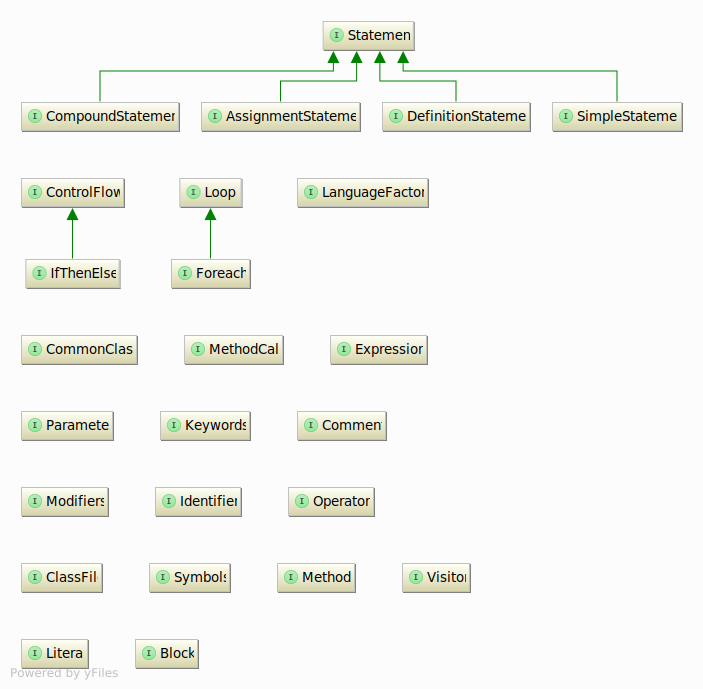
\includegraphics[width=\textheight]{resources/languagemodel_common}
    \caption{\textsc{Uml} Klassendiagramm des Zielsprachenmodells}
    \label{fig:language_model}
\end{sidewaysfigure}

Die Aufgabe des Generators ist die Transformierung des Applikationsmodells in das Modell der Zielsprache. 

Um die gewünschte Austauschbarkeit der Zielsprache zu gewährleisten wurde ein abstraktes Sprachenmodell entworfen welches die Konstrukte einer dateibasierten objektorientierten Programmiersprache (siehe \cref{sec:oo_languages}) abbildet. 
%Anforderungen erstellen und referenzieren.
Die gewünschte Zielsprache muss dabei die Klassen und Methoden des Modells implementieren sowie eine \emph{Language Factory} (siehe \cref{sec:language_factory}) bereitstellen um vom Generator genutzt werden zu können.
Um Semantik und Syntax der Zielsprache im Modell zu trennen --- abgesehen von Symbolen und Schlüsselwörtern --- wird die Syntax in der Klasse \emph{LanguageVisitor} (siehe \cref{sec:language_visitor}) gekapselt. Das Sprachenmodell kapselt somit die Semantik der Zielsprache.

Alle Interfaces des Modells (siehe \cref{fig:language_model}) erweitern das Interface \textbf{Visitor}. Somit ist sichergestellt, dass alle Klassen, die diese Schnittstellen implementieren, eine \emph{accept}-Methode für den \emph{LanguageVisitor} bereitstellen.

Basis des Modells ist das Interface \textbf{ClassFile}. Es abstrahiert eine Klassendatei mit den Eigenschaften:
\begin{compactitem}
    \item Dateiname
    \item Namensraum
    \item Liste von Abhängigkeiten (\emph{Dependency}-Klasse)
    \item Klassendefinition
\end{compactitem}

Die Liste von Abhängigkeiten der zu generierenden Klassen muss vorher aus dem Eingabemodell ermittelt werden. Dies geschieht durch Analyse der in den Elementdefinitionen des Schemamodells enthaltenen Typen. 

\textbf{Dependency} enthält das Schlüsselwort oder Methodenaufruf zum Import einer Quellcodedatei. In \textsc{Php} werden solche Dateien bpsw. so importiert: \texttt{require\_once("foo.php");}.

\textbf{Executable} implementieren alle Elemente der Zielsprache die \enquote{ausführbar} sind. Das Modell unterscheidet dabei zwischen \emph{Ausdruck} und \emph{Anweisung} (siehe \cref{sec:oo_languages}). 

Das Interface \textbf{CommonClass} dient der Implementierung einer Klassendefinition. Da das Interface selbst \emph{Statement} erweitert, kann eine Klasse weitere Klassendefinitionen beinhalten. Eine Klassendefinition besteht dabei aus einem Klassename, Modifiers und aus einer Menge von Statements:
\begin{compactitem}
    \item \emph{DefinitionStatement} zur Einführung von lokalen Variablen.
    \item \emph{Method} zur Definition von Methoden.
\end{compactitem}

Das \textbf{Modifier}-Interface deklariert Methoden um die Schlüsselwörter für \emph{Sichtbarkeitsmodifikatoren} (\enquote{Access Modifier}) und \enquote{Non Access Modifiers} wie \texttt{static} oder \texttt{final} zu erhalten.

Durch das \textbf{Method}-Interface kann eine Methodendefinition implementiert werden. Eine Methode beinhaltet dabei:
\begin{compactitem}
    \item Modifier
    \item Methodenname
    \item Rückgabetyp
    \item Liste von Parametern (Parameter können dabei alle Klassen sein die \emph{Expression} implementieren) % todo: liste von variablen, wie abstrahiert?
    \item \emph{Block}
\end{compactitem}

\textbf{Block} kapselt eine Menge von Statements.

Operatoren der Zielsprache müssen das Interface \textbf{Operator} implementieren, ein Operator ist durch seine Arität (Stelligkeit), Notation und sein Symbol gekennzeichnet. Zum Beispiel ist der Dereferenzierungsoperator in \textsc{Php} \emph{zweistellig}, \emph{Infix} notiert und durch das Symbol \texttt{->} gekennzeichnet.

\textbf{Keywords} und \textbf{Symbols} dienen zur Kapselung der Schlüsselwörter und Symbole einer Sprache. Keywords enthält Methoden zur Abfrage typischer Schlüsselworte wie \texttt{class}, \texttt{import}, \texttt{new} oder \texttt{this}. Sprachspezifische Symbole wie \emph{Verkettungs}- und \emph{Scope}-Operatoren oder Präfixe für Variablennamen können über Methoden der Klasse Symbols vom Generator abgefragt werden.

\subsubsection{Kompositum-Pattern im Sprachenmodell}
\label{sec:composite_pattern}

Zweck des Composite- oder auch Kompositum-Patterns ist die Gleichbehandlung von Einzel-
elementen und Elementgruppierungen in einer verschachtelten Struktur
(z. B. Baum), sodass aus Sicht des Clients keine explizite Unterscheidung
notwendig ist (nach \cite[][S. 102]{patternsKompakt}).

Anwendung fand das Pattern an zwei Stellen im Modell, erstens in den Klassen welche \textbf{Expression} und zweitens, welche \textbf{Statement} implementieren.
Ein Beispiel für den Aufbau eines Ausdrucks durch Klassen des Interface \emph{Expression} aus dem Sprachenmodell zeigt \cref{fig:example_expression}. Von \emph{Statement} abgeleitete Klassen können ebenso eine Baumstruktur bilden. \emph{Block} kann bspw. selbst wieder Codeblöcke --- also Statements vom Typ Block --- enthalten. 

\begin{figure}
    \[
        \overbrace{
            \underbrace{
                \overset{\text{Identifier}}{x} \underset{\text{Operator}}{+} \overset{\text{Identifier}}{y}
            }_{\text{SimpleExpression}} 
            \underset{\text{Operator}}{/}
            \underbrace{
                ( 
                    \underbrace{
                        \overset{\text{Literal}}{1.2} \underset{\text{Operator}}{*} \overset{\text{Literal}}{4}
                    }_{\text{SimpleExpression}} 
                )
            }_{\text{Group}}
        }^{\text{SimpleExpression}} 
    \]   
    \caption{Beispiel für den Aufbau einer \enquote{Expression} im Sprachenmodell}
    \label{fig:example_expression}
\end{figure}
